Medtech will integrate OpenEMR, a server and web application that will serve in back end operations. Since the problem is UI related, the solution is to simplify it into a usable product. We will use React to serve as the User Interface and redesign the UI into a user friendly interface. For users, they will be able to register and upon login, they will be displayed an overview with menus that can navigate to other tabs. To mitigate the problem of abundant tabs, a search engine will be implemented to be able to search for individual tabs or by category. The users will also be able to set their preferences on what they want to see upon startup, and set their own "category" view of what they want to see by selecting which tabs they want to see for one specific category, then can call up that category for calling up multible tabs.

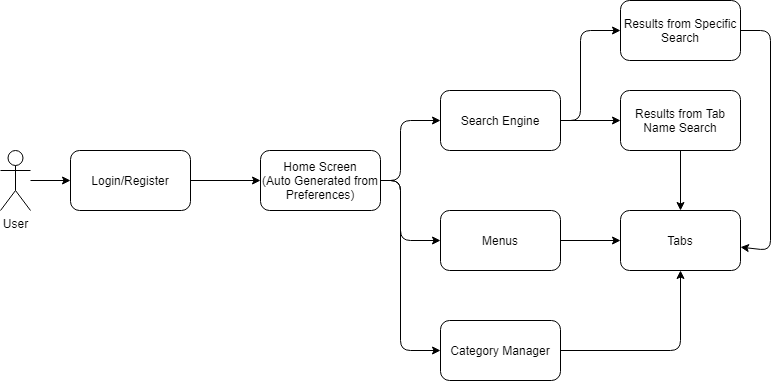
\includegraphics[width=1\textwidth]{images/use case 1.png}


Figure 1: Use Case showing interaction between user and application


For this application to be useful, we are planning on integrating a calender view for all the users. For nurses and docters, this will help plan out their work shift and for patients, it will keep track of all their appointments and potentially have events on calender when they have to take medicines when they are not at the hospital, to ease out the process.

This web application also needs to have a database that keep tracks of all patients and their individual profiles and health records. We are also planning on integrating a smart suggestion tool for medicine which medical professionals can use when prescribing medicines which will further cut their time spent on the computer. One of our main goals in this project is to help reduce the mental stress that medical professionals might experience in their initial practicing days by reducing the amount of information displayed at once and instead develop a smooth experience by giving only the information that they need.

We plan to integrate data from lab services as well through which labs can automatically send the reports through one email address and out product automatically attached that to its correct patient which prevents any further human intervention and help save time.

One of the pivotal feature of this product will be its analytical widgets. This will give doctors and nurses options to generate different helpful reports with a wide ranging spectrum starting from printing reports of how many on patients they need to perform medical check-up to their appointments. It will also have a feature that can generate graphs on different vitals of patient, like blood pressure and sugar level which can help identify trends and can lead to better patient care

